\documentclass[11pt]{amsart}

\usepackage[all]{xy}
\usepackage{amsmath}
\usepackage{amsfonts, mathrsfs}
\usepackage{amssymb}
\usepackage{amsthm}
\usepackage{mathtools}
\usepackage{enumerate,enumitem}
\usepackage{xcolor}
\usepackage{fullpage}
\usepackage{graphicx}
\usepackage{url}
\usepackage{caption}
\usepackage{csquotes}


\usepackage{hyperref}  
%\usepackage[notref,notcite]{showkeys}
\usepackage{tikz} 
\usepackage{tikz-cd}
\usepackage{comment}
\usetikzlibrary{arrows}
\usetikzlibrary{decorations.markings}
\usepackage{quiver}
\usepackage{changepage}

\theoremstyle{plain}
\newtheorem{theorem}{Theorem}[section]
\newtheorem{claim}[theorem]{Claim}
\newtheorem{lemma}[theorem]{Lemma}
\newtheorem{corollary}[theorem]{Corollary}
\newtheorem{conjecture}[theorem]{Conjecture}
\newtheorem{proposition}[theorem]{Proposition}

\theoremstyle{definition}

\newtheorem{remark}[theorem]{Remark}
\newtheorem{example}[theorem]{Example}
\newtheorem{definition}[theorem]{Definition}

\newcommand{\C}[1]{{\color{violet} #1}}


\DeclareMathOperator{\inc}{inc}
\DeclareMathOperator{\wt}{Wt}
\DeclareMathOperator{\Rep}{Rep}
\DeclareMathOperator{\Cir}{Cir}


\title{
Three dimensional toric varieties from quiver represenations
}

%\author{Mary Barker}
%\address{Department of Mathematics and Statistics,
%Washington University in St. Louis,
%One Brookings Drive, St. Louis, MO, 63130}
%\email{marybarker@wustl.edu}

%\author{Patricio Gallardo}
%\address{Department of Mathematics, 
%University of California, Riverside, CA, 92521}
%\email{pgallard@ucr.edu}  


\date{}


\begin{document}
\begin{abstract}
For a given dimension, there are only a finite number of toric varieties that emerge as moduli spaces of quiver representations with dimension vectors all equal to one. They are known as toric quiver varieties. In this work, we classify all the three-dimensional toric quiver varieties. Specifically, we demonstrate that there are five isomorphism classes among them, and that a single variation of GIT with 18 chambers is responsible for generating all of them. Additionally, we explore and describe the birational transformations between these varieties from both combinatorial and moduli theory perspectives.
\end{abstract}
\maketitle

\section{Updata Jan 15, 2025}

Questions that we are interested on
\begin{itemize}
    \item To generalize $\Gamma(Q)$ to the three dimensional polytope. So $\Gamma(Q) $ equal to $\Gamma(R)$ implies that flow polytopes with canonical weight are integrally affine isomorphic --or maybe affine integral isomorphic. 
    \item To compute, list and describe all the three-dimensional flow polytopes along with their invariants such as volume, $C(Q)$ and so forth
    \item[1.] To prove that adding a sink changes the polytope by cutting a corner.  
    \item To clean the writing of the three-dimensional case.
    \item Tightening for the three-dimensional case. 
\end{itemize}


\section{Introduction}

Understanding the geometry of moduli spaces and the objects parametrized by them is a central motivation in geometry. A particularly interesting case of such spaces is the moduli spaces of configurations of linear maps between vector spaces, supported on a directed graph. These objects, known as quiver representations, are important in representation theory and the birational geometry of varieties, as well as in applications to physics and even machine learning. Among all such moduli spaces, we focus on those where the linear maps are between one dimensional vector spaces and supported on an acyclic directed graph, see  subsection \ref{subsec:PrelQuives}.
These moduli spaces are called toric quiver varieties
and as their name suggests, they are projective toric varieties, and therefore each of them has an associated polytope. Due to work of \cite{domokos2016equations, altmann2009flow},  it is known that there is a finite number of toric quivers for a fixed dimension, as well as an algorithm to classify them. Yet, the classification is known explicitly only for dimension two.

In our first result, we completely described the three-dimensional projective toric quiver varieties, as well as their birational geometry. To describe our results we recall that given an acyclic directed graph $Q$ and a weight $\theta$ in their weights, there exist a moduli space of $\theta$-stable representations, also known as quiver representations.  This space is denoted as 
$M(Q, \theta)$ and its associated polytope (via toric geometry) is denoted as $\Delta(Q,\theta)$. By  \cite[Thm 4.22]{domokos2016equations}, 
for a fixed  dimension $d$, there is a set $\mathcal{R}_d$ of finite number of acyclic directed graphs such that any irreducible $d$-dimensional toric quiver variety is isomorphic to 
$M(Q, \theta)$ for some $\theta$ in $\mathcal{R}_d$.


\begin{theorem}\label{Thm:ThmA}
All toric quiver varieties of dimension two are isomorphic to one of the cases listed in Table
\ref{table:ListToricQuivers}. They are all related by a sequence of smooth blow ups at a point as follows:
\begin{align*}
    \xymatrix{
    \mathbb{P}^2  & \text{BL}_{pt}\mathbb{P}^2 \ar[l]
    & \text{BL}_{2pt}\mathbb{P}^2  \ar[l]  \ar[d]& 
    \text{BL}_{3pt}\mathbb{P}^2 \ar[l] 
    & 
    \\
    & &  \mathbb{P}^1 \times \mathbb{P}^1  & &      
    }
\end{align*}
\end{theorem}
Next, we describe a moduli interpretation of birational transformations among our spaces from their combinatorial interpretation.  In our first result, we provide both geometric and combinatorial information about these moduli spaces and their corresponding polytopes.
For a given quiver $Q$ and a weight $\theta$ at the vertices of $Q$, the toric quiver variety $X(\theta)$ parametrizes  $\theta$-stable representations supported on $Q$. As this moduli space is a projective toric variety, there exists an associated polytope $\Delta(\theta)$. This polytope parametrizes all $\theta$-stable, non-negative flow $(w_1,\ldots, w_6) \in (\mathbb{R}^6)_{\geq 0}$ supported on the quiver $Q$. The polytopes, as well as their transformations which mirror those from Theorem \ref{Thm:ThmA}, are depicted in Figure \ref{fig:Polytopes}.

\begin{figure}
    \centering
    
\includegraphics[scale = 0.2]{Polytopes}
    \caption{Polytopes $\Delta(\theta)$ associated to the toric varieties from Theorem \ref{Thm:ThmA}}
    \label{fig:Polytopes}
\end{figure}

We recall from Domokos \cite{domokos2016equations} that all two-dimensional toric quiver varieties can be obtained  from the quiver $Q$ shown in Figure \ref{fig:BipartiteQuiverK23}, by varying a weight $\theta$ . For a fixed weight $\theta$, the toric quiver variety is the moduli space $X(\theta)$, with the associated polytope $\Delta(\theta)$.

TO DO: 
\begin{itemize}
    \item To draw the dual graph of the chamber decomposition. So the vertices correspond to the chambers and they are joined only if they are share a codimension one wall.
    \item Can I check if two M(Q,theta) are in the same chamber, but calculating the stable rooted trees at the vertices? If they are the same. Then, they parametrize the same stable trees everywhere.
    \item I should write the code in a way the feeds from any quiver.
    \item Can I print the reference theta and read them?
    \item Can I print all the cones from the coneSystem and read them later?
    \item Can the code be parallelized by taking one hyperplane and spliting in two?
\end{itemize}


 
 


\begin{figure}[h!]
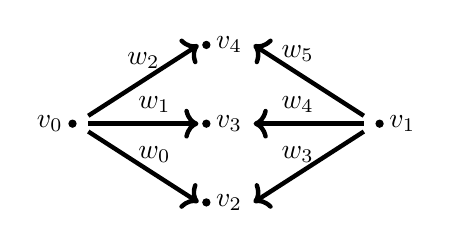
\begin{tikzpicture}[label/.style args={#1#2}{%
    postaction={ decorate,
    decoration={ markings, mark=at position #1 with \node #2;}}}]
\def\ra{0.5}
\def\rc{0.5}
\fill (-0.2 + \rc,1) circle (1.5pt) node[left] (A1) {$v_{0}$};
\fill (4.7- \rc,1) circle (1.5pt) node[right] (A2) {$v_{1}$};
\fill (2,0) circle (1.5pt) node[right] (B1) {$v_{2}$};
\fill (2,1) circle (1.5pt) node[right] (B2) {$v_{3}$};
\fill (2,2) circle (1.5pt) node[right] (B3) {$v_{4}$};
%
\draw[ ultra thick, label={0.6}{[above]{$w_0$}},-> ] 
(0+ \rc,0.9) -- (1.9,0);
\draw[ ultra thick, label={0.6}{[above]{$w_1$}},-> ] (0+\rc,1) -- (1.9,1);
\draw[ ultra thick, label={0.5}{[above]{$w_2$}},-> ] (0+\rc,1.1) -- (1.9,2);
\draw[ ultra thick, label={0.6}{[above]{$w_3$}},-> ] 
(4.5-\rc,0.9) -- (2.6,0);
\draw[ ultra thick, label={0.6}{[above]{$w_4$}},-> ] 
(4.5-\rc,1) -- (2.6,1);
\draw[ ultra thick, label={0.6}{[above]{$w_5$}},-> ] 
(4.5-\rc,1.1) -- (2.6,2);
\end{tikzpicture}
\caption{Bipartite quiver associated to $K_{2,3}$}
\label{fig:BipartiteQuiverK23}
\end{figure}



\begin{table}[!h]
\caption{
Toric quiver varieties, their respective chambers, as well  as key geometric and combinatorial information.
\ref{lemma:WallsDescription}
}
\label{table:ListToricQuivers}
\centering
\captionsetup[table]{skip=10pt}
\renewcommand{\arraystretch}{1.5} 
\begin{tabular}{|c|c|c|c|c|}
\hline
Toric variety & Chambers & rank Pic
& No Vertices polytope & Fano
\\ \hline
$\mathbb{P}^2$ & 3, 17 & 1 & 3 & Yes
\\ \hline
$\mathbb{P}^1 \times \mathbb{P}^1 $ 
& 
$0, 1, 2 $
& 2 & 4 & Yes
\\ \hline
$\text{BL}_{pt}\mathbb{P}^2$ & 
$4,5,7,13,15,16 $
& 2 & 4
& Yes
\\ \hline
$\text{BL}_{2pt}\mathbb{P}^2$ & 
$ 6,8,9,10,12,14 $
& 3 & 8
& Yes
\\ \hline
$\text{BL}_{3pt}\mathbb{P}^2$ & $11$  & 4 & 7
& Yes
\\ \hline
\end{tabular}
\end{table}


\section{Preliminaries}

\subsection{On toric varieties}


\subsection{On thin sincere quiver representations}
\label{subsec:PrelQuives}
A thin sincere representation of a quiver $Q$ assigns a one dimensional vector space to each vertex in $Q_0$ and a linear map to each arrow in $Q_1$.  
The space of all representations  of $Q$ is $\text{Rep}(Q) \cong \mathbb{C}^{Q_1}$, and their isomorphism classes are defined by action of $(\mathbb{C}^*)^{Q_0}$.   Representations of quivers have a notion of $\theta$-(semi)stability. Given a quiver $Q$ with weight $\theta \in C(Q)$, there is a projective complex toric variety 
$$
\overline{M}(Q, \theta) :=
Rep(Q) / \! \! /_{\theta} 
(\mathbb{C}^{*})^{|Q_0|-1}
$$
of dimension $|Q_1| - |Q_0| +1$ parametrizing $\theta$-semistable thin sincere representations up to isomorphism, see \cite{King1994} and \cite{Hille1998}. 

Given a representation
$ \omega$, we can define a subquiver $P := \text{Supp}(\omega)$ such that $P_0=Q_0$ and  $P_1 = \{ a \in Q_1 \;|\;  \omega(a) \neq 0 \}.$
This quiver is called the support of $\omega$, and $\omega$ is $\theta$-stable precisely when the subquiver 
$\text{Supp}(\omega)$ is $\theta$-stable, 
see  \cite[Lemma 1.4]{Hille1998} and discussion before \cite[Sec 2.2]{Altmann1999}.  Therefore, we can describe the $\theta$-stable and $\theta$-semistable representations parametrized by every $\overline{M}(Q,\theta)$.
 Moreover, via toric geometry, our package can be used to study these moduli spaces.
\begin{theorem}\cite{Hille1998}
If $\theta$ is in the interior of  $C(Q)$, the compact toric variety 
$\overline{M}(Q,\theta)$ is not empty and its associated polytope is 
equal to $\Delta(\theta)$. 
\end{theorem}

\section{Proof main results}

\begin{conjecture}
    
\end{conjecture}


\begin{theorem}\cite{domokos2016equations}
All toric quiver varieties of dimension two are isomorphic to \(\overline{M}(K_{2,3}, \theta)\) for some \(\theta\), where \(K_{2,3}\) is the quiver depicted in Figure \ref{fig:BipartiteQuiverK23}.
\begin{figure}[h!]
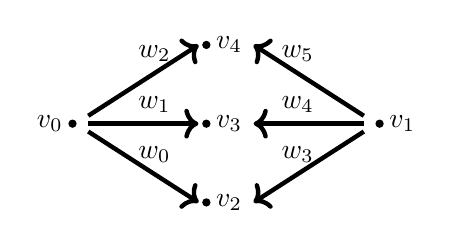
\begin{tikzpicture}[label/.style args={#1#2}{%
    postaction={ decorate,
    decoration={ markings, mark=at position #1 with \node #2;}}}]
\def\ra{0.5}
\def\rc{0.5}
\fill (-0.2 + \rc,1) circle (1.5pt) node[left] (A1) {$v_{0}$};
\fill (4.7- \rc,1) circle (1.5pt) node[right] (A2) {$v_{1}$};
\fill (2,0) circle (1.5pt) node[right] (B1) {$v_{2}$};
\fill (2,1) circle (1.5pt) node[right] (B2) {$v_{3}$};
\fill (2,2) circle (1.5pt) node[right] (B3) {$v_{4}$};
%
\draw[ ultra thick, label={0.6}{[above]{$w_0$}},-> ] 
(0+ \rc,0.9) -- (1.9,0);
\draw[ ultra thick, label={0.6}{[above]{$w_1$}},-> ] (0+\rc,1) -- (1.9,1);
\draw[ ultra thick, label={0.6}{[above]{$w_2$}},-> ] (0+\rc,1.1) -- (1.9,2);
\draw[ ultra thick, label={0.6}{[above]{$w_3$}},-> ] 
(4.5-\rc,0.9) -- (2.6,0);
\draw[ ultra thick, label={0.6}{[above]{$w_4$}},-> ] 
(4.5-\rc,1) -- (2.6,1);
\draw[ ultra thick, label={0.6}{[above]{$w_5$}},-> ] 
(4.5-\rc,1.1) -- (2.6,2);
\end{tikzpicture}
\caption{Bipartite quiver associated to $K_{2,3}$}
\label{fig:BipartiteQuiverK23}
\end{figure}
\end{theorem}

\begin{lemma}\label{lemma:WallsDescription}
The wall-chamber decomposition associated to the quiver $K_{2,3}$ has eighteen (top dimensional) chambers. They are represented in Figure ADD as follows: Each vertex corresponds to a maximal chamber, and two vertex share a vertex if and only if the corrresponding chamber share a codimension one wall. The labels on the vertex correspond to the cases in Table 1.    
\end{lemma}
\begin{proof}
    
\end{proof}

\begin{table}[h]
\centering
\caption{
Maximal chambers and their respective weights
}
\renewcommand{\arraystretch}{1.5} 
\label{your-table-label}
\begin{tabular}{| c | c | c | c | c | c|}
\hline
Maximal chambers & Weight $\theta$ & No Vertices & Lattice points & 
is Fano & Projective space
\\ \hline
0 & [-3, -3, 1, 1, 4] & 4 & 4 & True & False \\
1 & [-3, -3, 1, 4, 1] & 4 & 4 & True & False \\
2 & [-3, -3, 4, 1, 1] & 4 & 4 & True & False \\
3 & [-1, -5, 2, 2, 2] & 3 & 3 & True & True \\
4 & [-2, -5, 1, 3, 3] & 4 & 5 & True & False \\
5 & [-2, -5, 3, 1, 3] & 4 & 5 & True & False \\
6 & [-3, -5, 2, 2, 4] & 5 & 8 & True & False \\
7 & [-2, -5, 3, 3, 1] & 4 & 5 & True & False \\
8 & [-3, -5, 2, 4, 2] & 5 & 8 & True & False \\
9 & [-3, -5, 4, 2, 2] & 5 & 8 & True & False \\
10 & [-5, -3, 4, 2, 2] & 5 & 8 & True & False \\
11 & [-3, -3, 2, 2, 2] & 6 & 7 & True & False \\
12 & [-5, -3, 2, 2, 4] & 5 & 8 & True & False \\
13 & [-5, -2, 3, 1, 3] & 4 & 5 & True & False \\
14 & [-5, -3, 2, 4, 2] & 5 & 8 & True & False \\
15 & [-5, -2, 3, 3, 1] & 4 & 5 & True & False \\
16 & [-5, -2, 1, 3, 3] & 4 & 5 & True & False \\
17 & [-5, -1, 2, 2, 2] & 3 & 3 & True & True \\ \hline
\end{tabular}
\end{table}
\newpage




\section{Towards dimension three}


To generalize result from Theorem \ref{Thm:ThmA} to dimension three, we need a classification of three dimensional toric varieties. A first source is  \cite{batyrev1991classification}. It is known that there are 18 Fano cases, see \href{https://kasprzyk.work/research/pdf/GAELTalk.pdf}{Gael talk}. However, the Fano classification is not enough because there are toric quivers which are not Fano. 

\newcommand{\R}{\mathbb{R}}
\newcommand{\rs}{\mkern-12mu}

\newpage
\section{Tightening Quivers}

\begin{definition} \label{subquiver_weight}
    Consider a subgraph $P \subset Q$. Then, for a vertex $v \in P_0$, we define 
    \[
    \theta_P(v) := \sum_{\alpha \:\in\: P_1 \:|\: \alpha^+ = v}\rs \varepsilon(\alpha) - \sum_{\alpha \:\in\: P_1 \:|\: \alpha^- = v}\rs \varepsilon(\alpha).
    \]
    Naturally, if all edges incident to $v$ are in $P_1$, then $\theta_P(v) = \theta(v)$.
\end{definition}

\begin{definition}
    Let $G$ be the underlying undirected graph of some connected quiver $Q$, and let $v_1$, $v_2$, and $v_3$ be three vertices of $G$. Let $P$ be the subquiver of $Q$ defined by, in $G$, all paths from $v_1$ to $v_2$ not including $v_3$ and all subgraphs at most 1-connected to any vertex in these paths. Subgraphs connected to $v_1$. We say $P$ is the permutable subquiver induced by the vertices $v_1$ and $v_2$ without $v_3$.
    \newline
    If $R$ is a second permutable subquiver that is induced by $v_2$ and $w$ without $v_1$ and $P \cap R$ is exactly $v_2$, then we say $P$ and $R$ permute.
\end{definition}

\begin{proposition} \label{subquiver_permutation}
    Suppose $Q$ is a connected quiver and $v_1$, $v_2$, $v_3 \in Q_0$. Let $P \subset Q$ be a permutable subquiver induced by $v_1$ and $v_2$ without $v_3$ and $R \subset Q$ be another permutable subquiver induced by $v_2$ and $v_3$ without $v_1$. That is, $P$ and $R$ permute. This defines another (possibly disconnected) subquiver $Q^c$ by $Q^c_0 := (Q_0 \setminus (P_0 \cup R_0)) \cup \{v_1, v_3\}$ and $Q^c_1 := Q_1 \setminus (P_1 \cup R_1)$. Define $\widetilde{Q}$ to be the quiver with $P$ and $R$ in swapped locations maintaining orientation; that is, $\widetilde{Q}$ is the new (connected) quiver formed by first taking the disjoint union of $P$, $R$, and $Q^c$ and then identifying $v_1$ and $v_2$ in $P$ with $v_3 \in R$ and with $v_3 \in Q^c$, respectively, and identifying $v_2$ and $v_3$ in $R$ with $v_1 \in Q^c$ and $v_1 \in P$, respectively. Then, $\Delta(Q, \delta_Q)$ is integral-affinely isomorphic to $\Delta(\widetilde{Q}, \delta_{\widetilde{Q}})$
    
    
\end{proposition}

% Then, $\Delta(Q, \theta)$ is affinely isomorphic to $\Delta(\widetilde{Q}, \widetilde{\theta})$ where $\widetilde{\theta}$ is the new weight given by $\tilde{\theta}(u) = \theta(u) - \theta_P(u) + \theta_R(v)$, $\tilde{\theta}(v) = \theta(v) - \theta_P(v) - \theta_R(v) + \theta_P(u) + \theta_R(w)$, $\tilde{\theta}(w) = \theta(w) - \theta_R(w) + \theta_P(v)$ and $\tilde{\theta}(q) = \theta(q)$ for all other $q \in \widetilde{Q}_0 = Q_0$. In particular, $\Delta(Q, \delta_{\theta_Q})$ is integral-affinely isomorphic to $\Delta(\widetilde{Q}, \delta_{\theta_{\widetilde{Q}}})$.

\begin{proof}
    In progress
\end{proof}

\begin{comment}
    To begin, note the natural bijection $\varphi: Q_1 \to \widetilde{Q}_1$, given by sending $\alpha \in Q_1$ to $\tilde{\alpha}$ the edge's new location in $\widetilde{Q}_1$ which is well-defined by the construction of $\widetilde{Q}_1$. Also see that $\sum_{q \in Q_0}\tilde{\theta}(q) = 0$, so $\tilde{\theta} \in \mathbb{H_R}$. We assume that $\Delta(Q, \theta)$ is nonempty because otherwise either $\Delta(\widetilde{Q}, \tilde{\theta})$ is also empty, which would mean we are done, or $\Delta(\widetilde{Q}, \tilde{\theta})$ is nonempty in which case we can restart the proof and swap the roles of $\widetilde{Q}$ and $Q$. Finally, for a given tree $T$, we define the set $T^+_0(\alpha)$ (and $T^-_0(\alpha)$) as all vertices of $T_0$ that are connected to $\alpha^+$ (respectively $\alpha^-$) in the tree $T\setminus\{\alpha\}$.
    
    Suppose $T \subset Q$ is a $\theta$-stable spanning tree. We want to show there exists a spanning tree $\widetilde{T} \subset \widetilde{Q}$ that admits the same flow as T, as such trees correspond with a vertex in $\Delta(Q, \theta)$. By doing so, $\varphi$ a bijection means that there is a $\theta$-stable tree for every $\tilde{\theta}$-stable tree as well, both with the same flow, yielding $\Delta(Q, \theta) \cong \Delta(\widetilde{Q}, \tilde{\theta})$ as desired. 
    
    We can naturally construct a spanning tree $\widetilde{T} \subset \widetilde{Q}$ by taking $\tilde{\alpha}$ if $\alpha \in T_1$. Let $\tilde{\varepsilon}$ be the unique flow admitted by $\widetilde{T}$. For $\alpha \not\in T_1$, we get that $\tilde{\varepsilon}(\tilde{\alpha}) = \varepsilon(\alpha) = 0$. It then suffices to show $\tilde{\varepsilon}(\tilde{\alpha}) = \varepsilon(\alpha)$ for all $\alpha \in T_1$.
    
    Consider $\alpha \in T_1$ such that either $T^+_0(\alpha) \cap \{u, v, w\} = \varnothing$ or $T^-_0(\alpha) \cap \{u, v, w\} = \varnothing$. Then, $\tilde{\alpha}$ satisfies the same condition. Using that the flow of an edge is equivalent to the sum of the weights in $T^+_0(\alpha)$ or the negative of the sum of the weights in $T^-_0(\alpha)$ (as discussed at the start of Section 3 of \cite{hille2003quivers}, we have that 
    \[
    \tilde{\varepsilon}(\tilde{\alpha}) = \sum_{q \:\in\: \widetilde{T}^+_0(\tilde{\alpha})}\tilde{\theta}(q) = \sum_{q \:\in\: T^+_0(\alpha)}\theta(q) = \varepsilon(\alpha) \geq 0.
    \]
    where it is assumed in this case that $T^+_0(\alpha) \cap \{u, v, w\} = \varnothing$ was true. It can be shown that $\tilde{\varepsilon}(\tilde{\alpha}) = \varepsilon(\alpha)$ in a similar way if $T^-_0(\alpha) \cap \{u, v, w\} = \varnothing$ holds instead.

    Should the above condition not be true for some $\alpha$, then both $T^+_0(\alpha)$ and $T^-_0(\alpha)$ contain at least one vertex from $\{u, v, w\}$ because $P\cap R = \{v\}$ as in the hypothesis. In this case, we can choose either $T^+_0(\alpha)$ or $T^-_0(\alpha)$ and use the same identity from \cite{hille2003quivers} to equate $\tilde{\varepsilon}(\tilde{\alpha})$ to  $\varepsilon(\alpha)$ as done in the first case; however, the computation requires using at least one of the substitutions for $\tilde{\theta}(u)$, $\tilde{\theta}(v)$, or $\tilde{\theta}(w)$ given in the hypothesis depending on which vertices are in the subtree being considered. 

    To clarify the computation further, it is necessary to see that given a quiver $Q$ and weight $\theta \in \mathbb{H_R}$, any subquiver $\mathcal{O}$ (and thus any subtree) of $Q$ and weight $\theta_{\mathcal{O}} \in \R^{\mathcal{O}_0}$ defined for all $q \in \mathcal{O}_0$ by the equation in Definition \ref{subquiver_weight} will force $\theta_{\mathcal{O}} \in \mathbb{H_{R_{\mathcal{O}}}}$. This is because the image of the flow map $I_Q$ is exactly $\mathbb{H}_{\mathbb{R}_Q}$ and $I_{\mathcal{O}}(\pi(\varepsilon)) = \theta_{\mathcal{O}}$ for any flow $\varepsilon \in \R^{Q_1}$, where $\pi: \R^{Q_1} \to \R^{\mathcal{O}_1}$ is the projection given by keeping $\varepsilon(\alpha)$ if $\alpha \in \mathcal{O}_1$.  Intuitively, by removing the flow from edges outside the subquiver and adjusting the weights accordingly via the replacement $\theta(q) \mapsto \theta_{\mathcal{O}}(q)$ for all $q \in \mathcal{O}_0$, we have a well-defined \emph{quiver} whose weight on the vertices agrees with the flows on the edges.

    One way to show $\tilde{\varepsilon}(\tilde{\alpha}) = \varepsilon(\alpha)$ is to first let $\widetilde{T}^*$ equal $\widetilde{T}^+(\tilde{\alpha})$ or $\widetilde{T}^-(\tilde{\alpha})$, whichever has only one vertex from $\{u, v, w\}$ (which we will henceforth denote $\eta$) and $\tilde{\alpha}^* = \tilde{\alpha}^+$ or $\tilde{\alpha}^* = \tilde{\alpha}^-$ , whichever is in $T_0^*$. Then, partition the vertices of $T_0^*$ as follows. Define $\widetilde{X}_0$ as the set of all vertices besides $\eta$ that are connected to $\tilde{\alpha}^*$ through a path that does not include $\eta$ as a vertex. Also, define $\widetilde{Y}_0 := T^*_0\setminus (\widetilde{X}_0 \cup \{\eta\})$ so that $\widetilde{T}^*_0 = \widetilde{X}_0 \sqcup \{\eta\} \sqcup \widetilde{Y}_0$. 
    
    We can perform a similar decomposition on $T^*_0$ (which we set to be the same subtree as $\widetilde{T}^*_0$, e.g., if $\widetilde{T}^*_0 = \widetilde{T}^+_0(\tilde{\alpha})$ then $T^*_0 = T^+_0(\alpha)$). However, $T^*_0$ must contain two vertices from $\{u, v, w\}$ by construction of $\widetilde{Q}$ from $Q$; namely, $T^*_0$ must contain $\eta$ and another vertex $\xi \in \{u, v, w\}$, $\xi \neq \eta$. Moreover, the unique path from the vertex $\alpha^* = \alpha^+$ or $\alpha^* = \alpha^-$ (whichever is in $T^*_0$) to $\eta$ necessarily contains $\xi$ inside. Then, we partition $T^*_0$ like earlier but this time into three sets: $X_0 \subset T^*_0\setminus\{\xi\}$ all vertices connected to $\alpha^*$ through a path that does not contain $\xi$, $\mathcal{O}_0 \subset T^*_0\setminus \{\xi, \eta\}$ all vertices connected to both $\xi$ and $\eta$ through a path that does not pass through either of those vertices, and finally $Y_0 := T^*_0 \setminus (X_0 \cup \mathcal{O}_0 \cup \{\xi, \eta\})$ so that $T^*_0 = X_0 \sqcup \{\xi\} \sqcup \mathcal{O}_0 \sqcup \{\eta\} \sqcup Y_0$. The construction of these two partitions for $T^*_0$ and $\widetilde{T}^*_0$ guarantee that $\tilde{\theta}(q) = \theta(q)$ for all $q \in \widetilde{X}_0\cup\widetilde{Y}_0 = X_0\cup Y_0$. Moreover, if we let $X$, $\mathcal{O}$, and $Y$ be the induced subquivers $T^*[X_0\cup\{\xi\}]$, $T^*[\mathcal{O}_0\cup\{\xi, \eta\}]$, and $T^*[Y_0\cup\{\eta\}]$, respectively, we have
    \begin{equation}
        \theta(\xi) = \theta_{X}(\xi) + \theta_{\mathcal{O}}(\xi) \quad \text{ and } \quad \theta(\eta) = \theta_{\mathcal{O}}(\eta) + \theta_{Y}(\eta).
    \end{equation}
    which allows us to write
    \begin{align*}
        \varepsilon(\alpha) = \sum_{q \:\in\: T^*_0}\theta(q) &= \sum_{q \:\in\: X_0}\theta(q) + \theta(\xi) + \sum_{q \:\in\: \mathcal{O}_0}\theta(q) + \theta(\eta) + \sum_{q \:\in\: Y_0}\theta(q) \\
        &= \sum_{q \:\in\: X_0}\theta(q) + \theta_{X}(\xi) + \theta_{\mathcal{O}}(\xi) + \sum_{q \:\in\: \mathcal{O}_0}\theta(q) + \theta_{\mathcal{O}}(\eta) + \theta_{Y}(\eta) + \sum_{q \:\in\: Y_0}\theta(q) \\
        &= \sum_{q \:\in\: X_0}\theta(q) + \theta_{X}(\xi) + \theta_{Y}(\eta) + \sum_{q \:\in\: Y_0}\theta(q) \tag{2}
    \end{align*}
    where the weights on all vertices in the subquiver $\mathcal{O}$ vanished because $\theta_{\mathcal{O}} \in \mathbb{H_{R_{\mathcal{O}}}}$ and $\theta(q) = \theta_{\mathcal{O}}(q)$ for all $q \in \mathcal{O}_0$. Also note that there would be a negative sign in front of $\varepsilon(\alpha)$ if $T^* = T^-(\alpha)$ (which vanishes regardless since it would be in front of $\tilde{\varepsilon}(\tilde{\alpha})$ as well).
    
    We can write $\tilde{\varepsilon}(\tilde{\alpha})$ as the sum of the weights from $\widetilde{T}^*_0$ as well and get the following:
    \begin{align*}
        \tilde{\varepsilon}(\tilde{\alpha}) = \sum_{q \:\in\: \widetilde{T}^*_0}\tilde{\theta}(q) &= \sum_{q \:\in\: \widetilde{X}_0}\tilde{\theta}(q) + \tilde{\theta}(\eta) + \sum_{q \:\in\: \widetilde{Y}_0}\tilde{\theta}(q) \\
        &= \sum_{q \:\in\: X_0}\theta(q) + \tilde{\theta}(\eta) + \sum_{q \:\in\: Y_0}\theta(q)
    \end{align*}
    Note that by our construction of $\mathcal{O}$ and $Y$, $\mathcal{O}$ and $Y$ must be either of the subquivers $P$, $R$, or the complement of $T^*[P_0\cup R_0]$ contained in the subtree $T^*$. It can then be seen without much difficulty that by substituting $\tilde{\theta}(\eta)$ in the final equality above with its equivalent value stated in the hypothesis and then subsequently using (1) to replace $\theta(\eta)$, we can recover (2). Then, $\tilde{\varepsilon}(\tilde{\alpha}) = \varepsilon(\alpha)$, and we are done.
\end{comment}

\begin{proposition}\label{canonical-contraction-condition}
    (Joó-Domokos) Given a connected quiver $Q$ the pair $(Q, \delta_Q)$ is tight if and only if there is no partition $Q_0 = S \sqcup S'$ such that there is at most one arrow from $S$ to $S'$ and there is at most one arrow from $S'$ to $S$.
\end{proposition}

\begin{proposition}
    Given any connected quiver $Q$, $(Q, \delta_Q)$ can be made into a tight quiver $\widetilde{Q}$ such that $\Delta(Q, \delta_Q)$ is integral-affinely isomorphic to $\Delta(\widetilde{Q}, \delta_{\widetilde{Q}})$ via pruning, chain contraction, and subquiver permutation.
\end{proposition}

\begin{proof}
    We show that Proposition \ref{canonical-contraction-condition} holds only if we can find two permutable subquivers such that their permutation results in a quiver with an arrow contractable via either pruning or chain contraction.
    For the forward direction, suppose $Q_0 = S \sqcup S'$ with $\alpha$ an arrow from $S$ to $S'$ and possibly another arrow $\beta$ from $S'$ to $S$. Let $P \subset Q$ be the permutable subquiver induced by vertices $\alpha^-$ and $\beta^+$ without $\alpha^+$ if $\beta$ exists or by $\alpha^-$ and some $v \in S \setminus \{\alpha^-\}$ without $\alpha^+$ otherwise. Similarly, let $R \subset Q$ be the permutable subquiver induced by vertices induced by $\alpha^-$ and $\alpha^+$ without $\beta^+$ if $\beta$ exists or by $\alpha^-$ and $\alpha^+$ without $v$, otherwise. 
    
    By construction, $R$ is exactly the graph of the single edge $\alpha$ as any other undirected paths from $\alpha^-$ to $\alpha^+$ must go through $\beta^+$ (if it exists) since $\beta$ is the only edge besides $\alpha$ connecting $S$ and $S'$ by assumption. If $\beta$ does not exist, then $\alpha$ is a bridge, and so clearly no other undirected paths from $\alpha^-$ to $\alpha^+$ exist besides $\alpha$.
    
    In a similar way, $P$ is exactly the induced subgraph of the set of vertices in a tree incident to $\alpha^-$ or $\beta^+$ (or $v$ if $\beta$ does not exist). This follows from every edge in $Q[\hat{S}]$ being part of a path from $\alpha^-$ to $\beta^+$ or part of a tree incident to a non-terminal vertex in such a path. In the same way, any vertex in $S'$ cannot be part of a path from $\alpha^-$ to $\beta^+$ (or $v$ if $\beta$ does not exist) since any undirected path containing any vertex in $S'$ must necessarily contain $\alpha^+$.

    Notably, $P \cap R = \{\alpha^-\}$ and so $P$ and $R$ permute. Then, we can define $\widetilde{Q}$ as the resulting quiver after permuting $P$ and $R$ and apply Proposition \ref{subquiver_permutation} to see $\Delta(Q, \delta_Q)$ is integral-affinely isomorphic to $\Delta(\widetilde{Q}, \delta_{\widetilde{Q}})$. At this point, $\widetilde{Q}$ resembles one of the two cases below on the right. If $\beta$ exists, $\alpha$ can be contracted via chain contraction. Otherwise, pruning contracts $\alpha$. In either case, we result with a quiver that with the canonical weight produces a polytope integral-affinely isomorphic to $\Delta(Q, \delta_Q)$.
    \begin{figure}[h!]
        \centering
        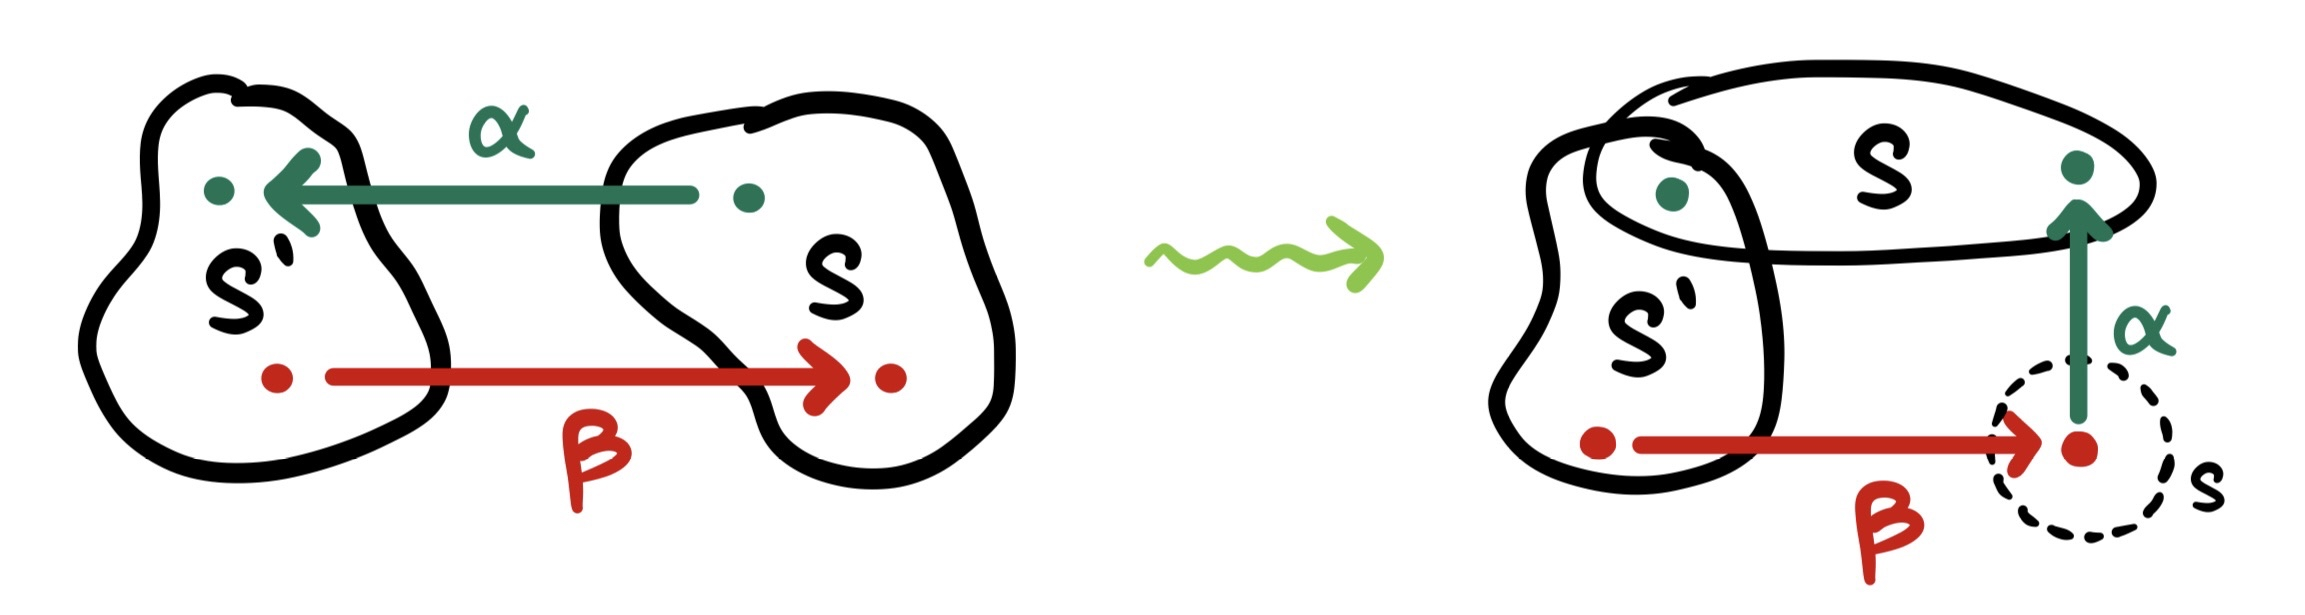
\includegraphics[width=0.75\linewidth]{permutationcase1.png}
    \end{figure}
    
    \begin{figure}[h!]
        \centering
        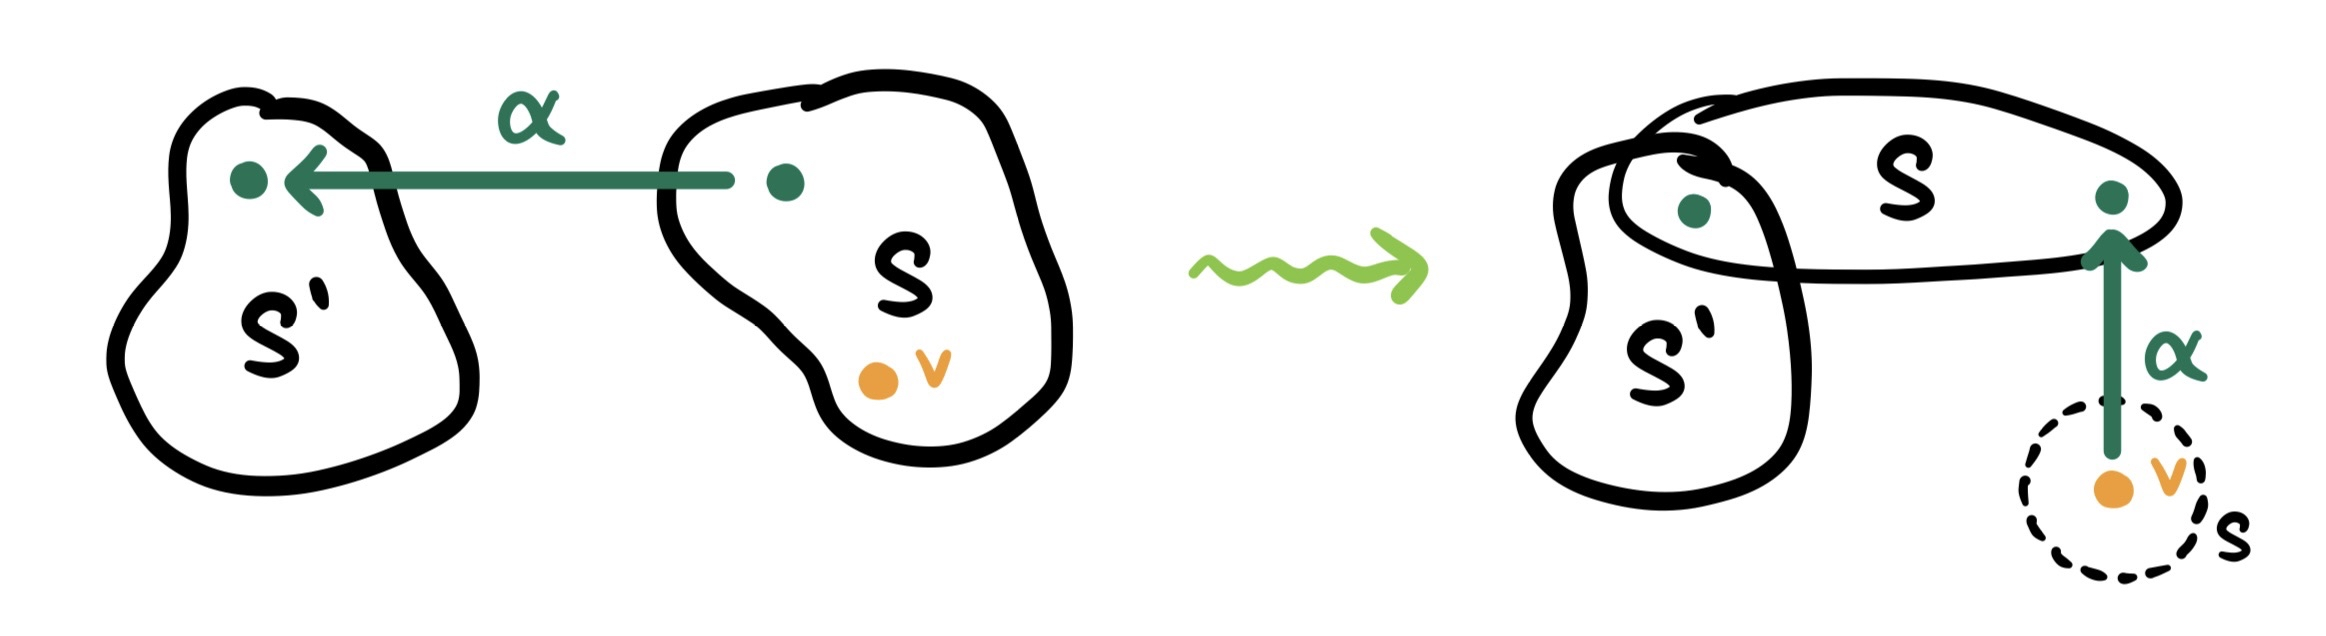
\includegraphics[width=0.75\linewidth]{permutationcase2.png}
    \end{figure}
    If there are more contractible arrows, then Proposition \ref{canonical-contraction-condition} holds and so we can perform subquiver permutation followed by pruning or chain contraction to contract the arrow as explained above. If no more contractible arrows exist, the quiver is tight.
\end{proof}

\end{document}

\newpage
\section{Extensions of trees and two-dimensional flow polytopes}

The polytope associated with a given quiver and weight can be determined by identifying all $\theta$-stable spanning trees of the quiver and calculating the regular flow of each that is admitted. This can be time-consuming depending on the quiver. In this section, we outline a method to easily determine, without calculation, the polytope of any two-dimensional quiver with the canonical weight. To do this, we first characterize  quivers as either ``disjoint" or ``nondisjoint" based on whether or not their two cycles share edges or not. Then, the polytope can be determined without difficulty as described in Theorems \ref{DisjointTreeExtension} and \ref{NondisjointTreeExtension}, the latter of which utilizes the tightening methods described in the previous section. Theorem \ref{DisjointTreeExtension} is immediate from Lemma \ref{cartesian_product_flow}, which was previously known (see Proposition 4.10 in \cite{domokos2016equations} ).

\begin{definition} \label{disjoint_def}
    Let $Q$ be a quiver of any dimension $d$. We say two cycles $C^1$ and $C^2$ of $Q$ are \textit{disjoint} if they share no edges; that is, 
    \[
        C^1_1 \cap C^2_1 = \varnothing
    \]
\end{definition} 

\begin{definition} 
    Let $G=(G_0, G_1)$ and $H = (H_0, H_1)$ be two disjoint graphs. We define 
    \[
    \mathcal{M}_{u,v}(G, H) := (G \sqcup H)/u \sim v
    \]
    as the new graph generated by identifying $u \in G_0$ with $v \in H_0$. 
\end{definition}

\begin{proposition} \label{decomposition_existence}
    Let $Q$ be a $d$-dimensional quiver with two disjoint cycles $C^1$ and $C^2$  with disjoint set of vertices. Let $G$ be the underlying graph of $Q$. Then, there exists two disjoint graphs $G'$ and $G''$ such that $C^1 \subset G'$ and $C^2 \subset G''$ and
    \[
    G = \mathcal{M}_{u,v}(G', G'')
    \]
    where $u \in G'_0$ and $v \in G''_0$.
** We can generalize when there is a cycle that is disjoint from the other ones **
\end{proposition}
\begin{proof}
** probably non- necessary ** 
%$C^1$ and $C^2$ are disjoint and thus share no edges. Since $G$ is connected, there exists two vertices $v_1 \in C^1_0$ and $v_2 \in C^2_0$ such that there exists a path $P$ that both connects $v_1$ to $v_2$ and that shares no edges with either cycle. Choose either $v_1$ or $v_2$ (we will choose $v_1$). Define the graph $G'$ as the union of all paths beginning at $v_1$ and whose edges incident to $v_1$ are in $C^1_1$. This graph is obviously connected and contains $C^1$. Define $G'' := G \setminus (G'\setminus \{v_1\})$. This graph is also connected since $G$ is connected and, furthermore, it contains $C^2$. The graphs $G'$ and $G''$ are disjoint because there exists no By construction, it also satisfies $G = \mathcal{M}_{u,v}(G', G'')$ as desired.
\end{proof}

\begin{proposition}\label{last_vertex_flow_equation}
** I don't understand that statement. Consider removing it ***
    Let $Q = (Q_0, Q_1)$ be a finite, acyclic quiver with $n$ vertices and $\theta \in \mathbb{H_R}$ be the weight. Let $u$ be some vertex in $Q_0$. Finally, let $\varepsilon \in \R^{Q_1}$ be a flow such that for all vertices $v \in Q_0 \setminus \{u\}$, the flow equation 
    \[
    \theta (v) = \sum_{\alpha \:|\: \alpha^+=\;v} \rs\varepsilon(\alpha) - \sum_{\alpha \:|\: \alpha^-=\;v}\rs\varepsilon(\alpha)
    \] 
    holds. Then 
    \[
    \theta(u) = \sum_{\alpha \:|\: \alpha^+=\;u}\rs\varepsilon(\alpha) - \sum_{\alpha \:|\: \alpha^-=\;u}\rs\varepsilon(\alpha)
    \] 
    holds as well and thus $I_Q(\varepsilon) = \theta$.
\end{proposition}

\begin{proof}
    Let $Q_0 = \{v_1, v_2, \dots, v_{n-1}, v_n = u \}$.
    By hypothesis, we have
    \begin{align*}
        \begin{dcases*}
            \theta (v_1) = \sum_{\alpha \:|\: \alpha^+=\;v_1}\rs\varepsilon(\alpha) - \sum_{\alpha \:|\: \alpha^-=\;v_1}\rs\varepsilon(\alpha) \\
            \theta (v_2) = \sum_{\alpha \:|\: \alpha^+=\;v_2}\rs\varepsilon(\alpha) - \sum_{\alpha \:|\: \alpha^-=\;v_2}\rs\varepsilon(\alpha) \\
            \quad \vdots \\
            \theta (v_{n-1}) = \sum_{\alpha \:|\: \alpha^+=\;v_{n-1}}\rs\rs \varepsilon(\alpha) - \sum_{\alpha \:|\: \alpha^-=\;v_{n-1}}\rs\rs \varepsilon(\alpha) \\
            \theta (u)= \varphi
        \end{dcases*}
    \end{align*}
    where $\varphi \in \R$ is the unknown value of the weight at the vertex $u$. Since $\theta \in \mathbb{H_R}$, we have that 
    \[
    \sum_{v \;\in\; Q_0}\theta(v) = 0.
    \]
    It follows immediately (by summing all of the equations from the system above) that 
    \begin{align*}
        \theta(v_1) + \cdots + \theta(v_{n-1}) + \theta(u) &= \sum_{\alpha \:|\: \alpha^+=\;v_1}\rs\varepsilon(\alpha) - \sum_{\alpha \:|\: \alpha^-=\;v_1}\rs\varepsilon(\alpha)
         + \cdots +  \sum_{\alpha \:|\: \alpha^+=\;v_{n-1}}\rs\rs \varepsilon(\alpha) - \sum_{\alpha \:|\: \alpha^-=\;v_{n-1}}\rs\rs \varepsilon(\alpha) + \varphi
    \end{align*}
    whereby
    \begin{align*}
         -\varphi &= \sum_{\alpha \:|\: \alpha^+=\;v_1}\rs\varepsilon(\alpha) - \sum_{\alpha \:|\: \alpha^-=\;v_1}\rs\varepsilon(\alpha)
         + \cdots +  \sum_{\alpha \:|\: \alpha^+=\;v_{n-1}}\rs\rs \varepsilon(\alpha) - \sum_{\alpha \:|\: \alpha^-=\;v_{n-1}}\rs\rs \varepsilon(\alpha). \tag{*}
    \end{align*}
    Now consider any $\alpha \in Q_1$. We have three cases.
    \begin{enumerate}
        \item[i.]  If $\alpha$ neither begins nor terminates at $u$, then every occurrence of $\varepsilon(\alpha)$ pairs with an occurrence of $-\varepsilon(\alpha)$ in the right hand side of (*).
        \item[ii.] If $\alpha$ terminates at $u$, then $\alpha^- = v_i$ for some $i \neq n$ (since $Q$ admits no loops) and $-\varepsilon(\alpha)$ occurs once in the right hand side of (*).
        \item[iii.] Similarly, if $\alpha$ begins at $u$, then $\alpha^+ = v_i$ for some $i \neq n$ and $\varepsilon(\alpha)$ occurs once in the right hand side of (*).
    \end{enumerate}
    Hence
    \[
        - \varphi = \sum_{\alpha \:|\: \alpha^+ = u} - \varepsilon(\alpha) + \sum_{\alpha \:|\: \alpha^- = u} \varepsilon(\alpha).
    \]
    
    %Recall that the flow equation sums over the flows $\varepsilon(\alpha)$ of all arrows $\alpha$ that either enter or exit some vertex in $Q_0$, adding the flows that enter and subtracting those that exit.
    %Consider an arrow $\alpha$ that enters some vertex $v \in Q_0 \setminus \{u\}$ and exits from another vertex $w \in Q_0 \setminus \{u\}$. Since we are summing over all vertices in $Q_0 \setminus \{u\}$ on the right-hand side of (1), then the flow of $\alpha$ contributes nothing to (1) because $\alpha$ enters some vertex $v \in Q_0 \setminus \{u\}$ and must necessarily exit another vertex $w \in Q_0 \setminus \{u\}$, causing the flows to annihilate eachother. We do not consider arrows where $v$ and $w$ are the same vertex because quivers with loops are not acyclic in the first place. 
    
    %Thus, the only arrows whose flows contribute to the right-hand side of (1) are those that either exit or enter the vertex $u$. These arrows must necessarily connect with some other vertex $v \in Q_0 \setminus \{u\}$, which is why the flow is included on the right-hand side of (1) in the first place. Importantly, these flows are not annihilated because one sum is missing from the right-hand side of (1), namely the sum that sums over all arrows entering and exiting the vertex $u$. Thus, the right-hand side is equal to the sum of all flows that enter or exit some vertex $v \in Q_0 \setminus\{u\}$ and that connect with $u$. It follows from (1) that $\varphi$ must equal exactly the negative of that so that the equation agrees. If we let $v$ be some vertex in $Q_0 \setminus \{u\}$, we have that
   % \begin{align*}
        %\varphi &= -\left(\sum_{\alpha \:|\: \alpha^+ =\;v,\; \alpha^- =\;u}\rs\rs\varepsilon(\alpha) - \sum_{\alpha \:|\: \alpha^- =\;v,\; \alpha^+ =\;u}\rs\rs\varepsilon(\alpha)\right) \\
        %&= \sum_{\alpha \:|\: \alpha^- =\;v,\; \alpha^+ =\;u}\rs\rs\varepsilon(\alpha) - \sum_{\alpha \:|\: \alpha^+ =\;v,\; \alpha^- =\;u}\rs\rs\varepsilon(\alpha) \\
        %&= \sum_{\alpha \:|\: \alpha^+ =\;u}\rs\varepsilon(\alpha) - \sum_{\alpha \:|\: \alpha^- =\;u}\rs\varepsilon(\alpha)
    %\end{align*}
    %where we can remove the condition in the final step that the arrow must connect with $v$ because $Q_0 \setminus \{u\}$ is the complement of $\{u\}$ and, similar to in the first case, loops cannot occur since $Q$ is acyclic. \\
\end{proof}

\begin{proposition}\label{existence_of_trees}
    If $T\cup\{\alpha, \beta\} = \mathcal{M}_{u,v}(T'\cup\{\alpha\}, T''\cup\{\beta\})$ for two vertices $u \in T'_0$ and $v \in T''_0$ and $S \subset T\cup\{\alpha, \beta\}$ is a spanning tree, then there exist two unique spanning trees $G' \subset T'\cup\{\alpha\}$ and $G'' \subset T''\cup\{\beta\}$ such that
    \[
        S = \mathcal{M}_{u,v}(G', G'').
    \]

\begin{proof}
    Take $G' = S \cap \left(T' \cup \{\alpha\}\right)$ and $G'' = S \cap \left(T'' \cup \{\beta\}\right)$ where $T' \cup \{\alpha\}$ and $T'' \cup \{\beta\}$ are naturally identified with subgraphs of $T \cup \{\alpha, \beta\}$.
    %First, note the edge set $T_1\cup\{\alpha, \beta\} = (T_1'\cup\{\alpha\})\sqcup(T_1''\cup\{\beta\})$. Let $E' = \{e \in S_1 \:|\: e \in T_1'\cup\{\alpha\}\}$ and $E'' = \{e \in S_1 \:|\: e \in T_1''\cup\{\beta\}\}$ be edge sets. Note that $E'\sqcup E'' = S_1$. Next, define the graphs $G' = (T_0', E')$ and $G'' = (T_0'', E'')$. Naturally, $G'$ and $G''$ have no loops and are connected since their edge sets come from the edges of $S$, a connected tree, in the first place. By construction, $G'$ and $G''$ connect to all vertices in $T'\cup\{\alpha\}$ and  $T''\cup\{\beta\}$, respectively. They are thus both spanning trees with respect to the graphs $T'\cup\{\alpha\}$ and  $T''\cup\{\beta\}$. Since $G'$ must then connect to vertex $u$ and $G''$ must connect to vertex $v$, then $\mathcal{M}_{u,v}(G', G'')$ is well-defined and connected with vertex set $T_0$ and edge set $S_1$. The graph $\mathcal{M}_{u,v}(G', G'')$ is also still a spanning tree since $\mathcal{M}_{u,v}$ only connects the graphs at one point. Thus, no new loops can form. Recalling that $S_0 = T_0$ since $S$ is a spanning tree, then $\mathcal{M}_{u,v}(G', G'')$ is isomorphic to $S$ since they have the same vertex and edge sets. Moreover, the two trees are unique because any spanning trees $\Tilde{G}'$ and $\Tilde{G}''$ must have the same vertex and edge set as graphs $G'$ and $G''$ due to the construction described above. Then, $\Tilde{G}'$ and $\Tilde{G}''$ are automatically isomorphic to $G'$ and $G''$, respectively. Thus, $G'$ and $G''$ are unique.
\newline
\end{proof}
    
\end{proposition}

\begin{definition}
Recall that given a flow $\epsilon$, its support is the set of arrows such that $\epsilon(\alpha) \neq 0$, we consider the set: 
    \begin{align*}
     \Lambda(Q, \theta) = \bigg\{
    \varepsilon \in I_Q^{-1}(\theta) \; | \text{ there is a spanning tree $T$ with a regular flow such that $Supp(\epsilon) \subset T$}
     \bigg\}
    \end{align*}
\end{definition}

\begin{remark}
    %(Is this true? This is my understanding.) \color{blue}{[not sure, Patricio says it's true for a general weight, not being on a wall]} \color{black}
     There is a bijection between $\Lambda(Q, \theta)$ and the set of vertices of $\Delta(Q, \theta)$ ** WARNING: the moduli interpretation breaks if we are working with $\theta$ in the wall. Is this claim true? ** However, there is not necessarily a bijection between the set of spanning trees of $Q$ that admit regular flows and $\Lambda(Q, \theta)$ (although, by definition, the former surjects onto the latter). In other words, there may be multiple spanning trees of $Q$ that share the same regular flow, but they correspond to a single element of $\Lambda(Q, \theta)$ and are thus realized as a single vertex in the associated polytope ** EXAMPLE ** 
\end{remark}

\begin{remark} \label{1-to-1-edges}
    Each edge $e \in T_1\cup\{\alpha, \beta\}$ can be associated with a unique edge in either $T_1'\cup\{\alpha\}$ or $T_1''\cup\{\beta\}$, but not both, based on the structure (valencies of connected vertices, etc.) of the graphs alone (the flow $\varepsilon$ has no effect on this association). This is simply because $T_1' \cup \{\alpha\}$ and $T_1'' \cup \{\beta\}$ are naturally identified with subgraphs of $T_1 \cup \{\alpha, \beta\}$.
\end{remark}
%May require additional detail using a map/isomorphism or something} 

\begin{lemma} \label{cartesian_product_flow}
    If $T\cup\{\alpha, \beta\} = \mathcal{M}_{u,v}(T'\cup\{\alpha\}, T''\cup\{\beta\})$ for two vertices $u \in T'_0$ and $v \in T''_0$, then 
    \[
    \Lambda(T\cup\{\alpha, \beta\}, \delta_\theta) = \Lambda(T'\cup\{\alpha\}, \delta_{\theta_{T'}}) \times \Lambda(T''\cup\{\beta\}, \delta_{\theta_{T''}})
    \]
    where $\delta_\theta$, $\delta_{\theta_{T'}}$, and $\delta_{\theta_{T''}}$ are the canonical flows for $T\cup\{\alpha, \beta\}$, $T'\cup\{\alpha\}$, and $T''\cup\{\beta\}$, respectively.
\end{lemma}

\begin{proof}
We show $\Lambda(T\cup\{\alpha, \beta\}, \delta_\theta) \subseteq \Lambda(T'\cup\{\alpha\}, \delta_{\theta_{T'}}) \times \Lambda(T''\cup\{\beta\}, \delta_{\theta_{T''}})$. The reverse containment is similar.

Assume that $T'\cup\{\alpha\}$ has $n$ edges and $T''\cup\{\beta\}$ has $m$ edges so that $T\cup\{\alpha, \beta\}$ has $n + m$ edges.
%since $T\cup\{\alpha, \beta\} = \mathcal{M}_{u,v}(T'\cup\{\alpha\}, T''\cup\{\beta\})$.
Let $\varepsilon = (\varepsilon_1, \varepsilon_2, \ldots, \varepsilon_{n+m})$ where $\varepsilon \in \Lambda(T\cup\{\alpha, \beta\}, \delta_\theta)$ and each component $\varepsilon_i$ of $\varepsilon$ is the flow of the edge $e_i \in T_1\cup\{\alpha, \beta\}$.
%\color{red}{*}\color{black}
We may relabel edges so that $\varepsilon = x \times y$ where $x = (x_1, ..., x_n)$ and $y = (y_1, ..., y_m)$ are flows on $T'\cup\{\alpha\}$ and $T''\cup\{\beta\}$, respectively. We will show that $x \in \Lambda(T'\cup\{\alpha\}, \delta_{\theta_{T'}})$ and $y \in \Lambda(T''\cup\{\beta\}, \delta_{\theta_{T''}})$. In order for this to occur, three conditions must hold:
\newline
\begin{enumerate}
    \item Both $x$ and $y$ must be regular flows.
    \item There must exist spanning trees $S' \subset T'\cup\{\alpha\}$ and $S'' \subset T''\cup\{\beta\}$ such that $x_j=0$ whenever $x_j$ is the flow of some edge $e' \not\in S_1'$ and $y_k=0$ whenever $y_k$ is the flow of some edge $e'' \not\in S_1''$.
    \item $I_{T'\cup\{\alpha\}}(x) = \delta_{\theta_{T'}}$ and $I_{T''\cup\{\beta\}}(y) = \delta_{\theta_{T''}}$.
\end{enumerate} \leavevmode \newline
%To verify these three conditions,
Consider the isomorphism
\begin{align*}
    \zeta : \R^n \times \R^m &\longrightarrow \R^{n+m} \\
    (x, y) &\mapsto \varepsilon 
\end{align*}

%%%
\iffalse
where $\zeta$ is defined by
\begin{equation*}
    \varepsilon_i = 
    \begin{dcases*}
        x_j,\quad \text{when} \;e_i\; \text{corresponds to the edge}\; e'_j \in  T_1'\cup\{\alpha\} \\
        y_k,\quad \text{when} \;e_i\; \text{corresponds to the edge}\; e''_k \in  T_1''\cup\{\beta\}
    \end{dcases*}
\end{equation*}
where $e_i \in T_1\cup\{\alpha, \beta\}$ is the edge with flow $\varepsilon_i$, $x_j$ and $y_k$ are the flows of the edge $e'_j$ and $e''_k$, respectively (note that the ordering of the edges can always be reordered to match the ordering of the flows so that flow $\varepsilon_i$ is the flow of edge $e_i$ for all $i$), and $1 \leq i \leq n+ m$, $1 \leq j \leq n$, and $1 \leq k \leq m$. The map $\zeta$ is invertible since $T_1'\cup\{\alpha\}$ and $T_1''\cup\{\beta\}$ are disjoint and due to Remark \ref{1-to-1-edges}.
\fi
%%%%%%

%We now return to the conditions.
\noindent Since $\varepsilon \in \Lambda(T\cup\{\alpha, \beta\}, \delta_\theta)$, there exists a spanning tree $S \subset T\cup\{\alpha, \beta\}$ which supports the regular flow $\varepsilon$. 
%By definition of \textit{admitting} a flow,
Hence $\varepsilon_i = 0$ if the corresponding edge $e_i \not\in S_1$ and $\varepsilon_i \geq 0$ if the corresponding edge $e_i \in S_1$.
Let $(x,y) = \zeta^{-1}(\varepsilon)$. By Proposition \ref{existence_of_trees}, there exist two unique spanning trees $S' \subset T'\cup\{\alpha\}$ and $S'' \subset T''\cup\{\beta\}$ such that $S = \mathcal{M}_{u,v}(S', S'')$.
Conditions (1) and (2) then hold immediately.
%Because $S_1 = S_1'\sqcup S_1''$, if $x_j$ is the flow corresponding to an edge $e_j' \in S_1'$, then $e_j' \in S_1$ which implies $x_j \geq 0$. Then, condition (1) is met for flow $x$. Similarly, if $x_j$ is the flow corresponding to an edge $e_j' \not\in S_1'$, then $e_j' \not\in S_1$ since the edge is not in $T_1''\cup\{\beta\}$ by definition of $\zeta$. Then, $x_j = 0$ only if $e_j \not\in S_1'$. Condition (2) is now met for $x$. The same exact argument can be used to verify conditions (1) and (2) for flow $y$ but with $S''$ instead.
For condition (3) to be met for $x$, the flow equation 
\[
    \delta_{\theta_{T'}}(q') = \sum_{e' \:|\: e'^+=\;q'} \rs x(e') - \sum_{e' \:|\: e'^-=\;q'}\rs x(e')
\]
must hold for all vertices $q' \in T_0'$, where $e'$ denotes an edge in $T_1'\cup\{\alpha\}$.  For the condition to hold for $y$, the same equation must hold for all vertices $q'' \in T_0''$ and edges $e'' \in T_1''\cup\{\beta\}$. Noting that $\varepsilon \in \Lambda(T\cup\{\alpha, \beta\}, \delta_\theta)$, we have 
\[
    \delta_{\theta_{T}}(q) = \sum_{e \:|\: e^+=\;q} \rs\varepsilon(e) - \sum_{e \:|\: e^-=\;q}\rs\varepsilon(e)
\]
for all vertices $q \in T_0$ where $e$ denotes an edge in $T_1\cup\{\alpha,\beta\}$. Let $w \in T_0$ denote the vertex that is formed by identifying $u$ and $v$ via $\mathcal{M}_{u,v}$.
%If $q \neq w$ and $q' \neq u$, then $\delta_{\theta_{T}}(q) = \delta_{\theta_{T'}}(q')$ where $q'$ in the subgraph $T'\cup\{\alpha\}$ corresponds to the vertex $q$ in the original graph $T\cup\{\alpha, \beta\}$. Similarly, if $q$ corresponds to $q''$, $\delta_{\theta_{T}}(q) = \delta_{\theta_{T''}}(q'')$ if $q \neq w$ and $q' \neq v$.

When considering the canonical weight, the weight of each vertex is equal to the number of incoming edges minus the number of outgoing edges.
The map $\mathcal{M}_{u,v}$ does not affect the valency of any vertex other than $u$ and $v$ (which become the vertex $w$), so the canonical weight is consistent with $\delta_{\theta_{T}}(q)$, $\delta_{\theta_{T'}}(q')$, and $\delta_{\theta_{T''}}(q'')$ so long as $q \neq w$, $q' \neq u$, and $q'' \neq v$.
Moreover, only $w$ is adjacent to edges that are present in both $T'\cup\{\alpha\}$ and $T''\cup\{\beta\}$. Thus all weights excluding those of $u$, $v$, and $w$ are unchanged by $\mathcal{M}_{u,v}$. Note that flows are preserved by $\mathcal{M}_{u,v}$. Hence the flow equation automatically holds for all vertices excluding $u$, $v$, and $w$.

To show that the flow equation holds for the remaining vertices, note that all vertices in $T'\cup\{\alpha\}$ aside from $u$ satisfy the flow equation.
%\color{purple}(Once again, I believe there is another way to show the next step without Prop 5.4)\color{black}
Then by Proposition \ref{last_vertex_flow_equation}, the flow equation must necessarily hold for $u$ as well because $\delta_{\theta_{T'}} \in \mathbb{H_R}$ by assumption. The same argument holds for $v$. Thus condition (3) is met and we have $x \in \Lambda(T'\cup\{\alpha\}, \delta_{\theta_{T'}})$ and $y \in \Lambda(T''\cup\{\beta\}, \delta_{\theta_{T''}})$.

%To show backward containment, the proof follows many of the same arguments but in the opposite direction. 

%\color{red}{* May require additional detail using a map/isomorphism or something}\color{black}
\end{proof}

\begin{theorem} \label{DisjointTreeExtension}
    $\Delta(T\cup\{\alpha,\beta\}, \delta_\theta)$ is affinely isomorphic to a square if and only if $\alpha$, $\beta$ are two disjoint arrows in $T\cup\{\alpha,\beta\}$.
\end{theorem}

\begin{proof}
If $\alpha$ and $\beta$ are disjoint, then by Proposition \ref{decomposition_existence}, $T\cup\{\alpha, \beta\}$ can be expressed as the merging of two quivers $T'\cup\{\alpha\}$ and $T''\cup\{\beta\}$ via $\mathcal{M}_{u,v}$.

Note $\dim\Delta(T'\cup\{\alpha\}, \delta_{\theta_{T'}}) = \dim\Delta(T''\cup\{\beta\}, \delta_{\theta_{T''}}) = 1$ and thus both polytopes are isomorphic to line segments, which are each defined by two vertices. Then, $|\Lambda(T'\cup\{\alpha\}, \delta_{\theta_{T'}})| = |\Lambda(T''\cup\{\beta\}, \delta_{\theta_{T''}})| = 2$. It follows that $|\Lambda(T'\cup\{\alpha\}, \delta_{\theta_{T'}}) \times \Lambda(T''\cup\{\beta\}, \delta_{\theta_{T''}})| = 4$. Note that $\Lambda(T'\cup\{\alpha\}, \delta_{\theta_{T'}}) \times \Lambda(T''\cup\{\beta\}, \delta_{\theta_{T''}}) = \Lambda(T\cup\{\alpha, \beta\}, \delta_\theta)$ by Lemma \ref{cartesian_product_flow}. Then, $\Delta(T\cup\{\alpha, \beta\}, \delta_\theta)$ has four vertices. 

We know that $\dim\Delta(T\cup\{\alpha, \beta\}, \delta_\theta) = 2$. Hence $\Delta(T\cup\{\alpha, \beta\}, \delta_\theta)$ is a square. The converse follows from the complete two-dimensional classification of Theorem \ref{NondisjointTreeExtension}.
\newline
\end{proof}

\newcommand{\Pa}{P_{\alpha}}
\newcommand{\Pb}{P_{\beta}}

From this point forward, we denote $\Pa := C(T, \alpha) \setminus \{\alpha\}$ and $\Pb := C(T, \beta) \setminus \{\beta\}$. We now define the notion of a 'pruned' tree in order to greatly reduce the complexity of the remaining tree-extension quivers we have to consider.

\begin{definition}
Let $Q$ be a quiver of dimension $n$ (so it has $n$ cycles). Then $Prune(Q)$ is the smallest connected subquiver of $Q$ that contains all the cycles of $Q$.



\textbf{Old one}
    Let $T\cup\{\alpha, \beta\}$ be a well-defined tree-extended quiver. If $\alpha$ and $\beta$ are not disjoint, then $\text{pruned}(T) := \Pa \cup \Pb$. Otherwise, $\text{pruned}(T) := \Pa \cup \Pb \cup R$, where $R \subset T$ is the unique path connecting $\Pa$ and $\Pb$. Then, we can define the pruned tree-extension $\text{pruned}(T)\cup\{\alpha, \beta\}$ constructed by appending $\alpha$ and $\beta$ to the same vertices as in $T\cup\{\alpha, \beta\}$. We note appending them at these locations in the pruned tree is always possible because $\alpha^+, \alpha^- \in \Pa$ and $\beta^+, \beta^- \in \Pb$.
\end{definition}

\begin{proposition} \label{pruning}
    Given a $\;T\cup\{\alpha, \beta\}$ and $\; \widetilde{T}\cup\{\alpha, \beta\}$ where $\widetilde{T} := \text{\emph{pruned}}(T)$, then $\Delta(\widetilde{T}\cup\{\alpha, \beta\}, \delta_{\theta_{\widetilde{T}}})$ is affinely isomorphic to $\Delta(T\cup\{\alpha, \beta\}, \delta_{\theta})$.
\end{proposition}

\begin{proof}
    Suppose $\widetilde{T}\cup\{\alpha, \beta\}$ has $n$ vertices. Note that $\widetilde T$ is naturally a subgraph of $T$. For each vertex $\tilde{v}_i$ in $\widetilde{T}$, consider the corresponding vertex $v_i$ in the original graph $T\cup\{\alpha, \beta\}$. Let $S^i$ be the union of all subgraphs of $T$ containing $v_i$ that share no edges with $\widetilde T$. We note that one may obtain $S^i_1 = \{v_i\}$ in which case $S^i$ is omitted from consideration.

    If the trees $S^1, \ldots, S^n$ are defined as outlined above, then it is not difficult to see that
    \[
        T\cup\{\alpha, \beta\} = M_{\tilde{v}_n, v_n}(\ldots M_{\tilde{v}_2, v_2}(M_{\tilde{v}_1, v_1}(\widetilde{T}\cup\{\alpha, \beta\}, S^1), S^2) \ldots ,S^n).
    \]
    By Lemma \ref{cartesian_product_flow}, we have
    \begin{equation*}
    \Lambda(T\cup\{\alpha, \beta\}, \delta_{\theta}) = \left(\left(\left(\Lambda(\widetilde{T}\cup\{\alpha, \beta\}, \delta_{\theta_{\widetilde{T}}}) \times \Lambda(S^1, \delta_{\theta_{S^1}})\right)
    \times \Lambda(S^2, \delta_{\theta_{S^2}})\right)
    \cdots \times \Lambda(S^n, \delta_{\theta_{S^n}})\right)
    \end{equation*}
    Since we repeatedly merged with only trees---which admit exactly one unique flow---each successive Cartesian product does not alter the shape nor the number of vertices of the polytope of the resulting graph. Hence $\Delta(\widetilde{T}\cup\{\alpha, \beta\}, \delta_{\theta_{\widetilde{T}}})$ is affinely isomorphic to $\Delta(T\cup\{\alpha, \beta\}, \delta_{\theta})$.
\end{proof}

\begin{proposition}
    Suppose $Q = T \cup \{\alpha_1, \alpha_2, \dots , \alpha_n\}$ has $n$ disjoint cycles. Then $\Delta(Q, \delta_\theta)$ is a hyper-rectangle. 
\end{proposition}

\begin{proof}
    There is a sequence of subquivers $Q_1, Q_2 \dots, Q_m$ of $Q$ and pairs of vertices $\{(u_i, v_i) \ : \ i = 1, 2, \dots, m\}$ of these subquivers such that 
    \[
        Q = M_{u_m, v_m}( \cdots M_{u_2, v_2}(M_{u_1, v_1}(Q_1, Q_2), Q_3),\dots, Q_m)
    \]
    where each $Q_i$ is either a tree, which admits a unique flow, or a tree up to removing some $\alpha_k$, whose flow polytope is a line segment. Lemma \ref{cartesian_product_flow} yields
    \[
        \Lambda(Q, \delta_{\theta_{Q}}) = \Lambda(Q_1, \delta_{\theta_{Q_1}}) \times \Lambda(Q_2, \delta_{\theta_{Q_2}}) \times \cdots \times \Lambda(Q_m, \delta_{\theta_{Q_m}})
    \]
    whereby $\Delta(Q, \delta_\theta)$ is necessarily a hyper-rectangle.
\end{proof}




We now begin the classification of ``nondisjoint'' two-dimensional tree extensions, that is, all tree-extended quivers that do not satisfy the conditions to be disjoint outlined in Definition \ref{disjoint_def}.

\begin{proposition} \label{deg_three_vertices}
A two-dimensional quiver $Q$ has two non-disjoint cycles, $C_1$ and $C_2$, (see Definition \ref{disjoint_def}.) if and only if there are exactly two vertices $\nu_1$ and $\nu_2$ with three incident edges in  $Prune(Q)$. Moreover, $\nu_1$ and $\nu_2$ are the terminal vertices of the path $P_{\alpha}\cap P_{\beta}$.


%    Consider a two-dimensional tree extension $T\cup\{\alpha, \beta\}$. The appended arrows $\alpha$ and $\beta$ and let $C_{\alpha}$ and $C_{\beta}$ be the cyclic with the least number of edges such that $\alpha \in C_{\alpha}$    and $\beta \in C_{\beta}$.
%$\text{\emph{pruned}}(T)\cup\{\alpha, \beta\}$. 



\end{proposition}

\begin{proof}
    We consider the graph $\emph{pruned}(T)\cup\{\alpha, \beta\}$ since the only edges and vertices that matter in the hypothesis are from this subgraph.

    Since $\alpha$ and $\beta$ are nondisjoint---that is, $C(T, \alpha)_1 \cap C(T, \beta)_1 \neq \varnothing$---there exists a path $\Pa \cap \Pb$ in $T\cup\{\alpha, \beta\}$. The terminal vertices of this path must be of valency 3, with one edge from each of $P_\alpha \cap P_\beta$, $C(T, \alpha)$, and $C(T, \beta)$.
    %because at these vertices the graph diverges to connect to the two cycles $C(T, \alpha)$ and $C(T, \beta)$. If the graph does not diverge at that terminal vertex, then incident edge not in $\Pa \cap \Pb$ (which must exist since the vertex is terminal and leaves are pruned in $\emph{pruned}(T)\cup\{\alpha, \beta\}$) has to be in both cycles, which means it is in $\Pa \cap \Pb$.
    These terminal vertices cannot have valency 4 or greater because any additional edges must necessarily connect somewhere else in the graph (since leaves are pruned) creating an additional cycle in the graph which cannot occur. For the same reason, all other vertices have valency $2$.
\newline
\end{proof}

\begin{definition} \label{gamma_number}
    Count the number of traversable paths from $\nu_1$ to $\nu_2$ and from $\nu_2$ to $\nu_1$. From this point forward, we let $\nu_1$ be the vertex that has more traversable paths to $\nu_2$. Define $\Gamma(Q)$ to be the number of traversable paths from $\nu_1$ to $\nu_2$ in a tree-extended quiver $Q$.
\end{definition}

\begin{corollary} \label{gamma_bounds}
    For any nondisjoint two-dimensional tree extension $T\cup\{\alpha, \beta\}$, 
    \[
    0 \leq \Gamma(T\cup\{\alpha, \beta\}) \leq 3.
    \]
\end{corollary}

\begin{proof}
    Immediate from Proposition \ref{deg_three_vertices} and the definition of $\Gamma$ since $\nu_1$ and $\nu_2$ have 3 incident edges in $\text{\emph{pruned}}(T)\cup\{\alpha, \beta\}$, and a walk starting at $\nu_1$ or $\nu_2$ towards any of these incident edges cannot lead to a leaf since $\text{\emph{pruned}}(T)\cup\{\alpha, \beta\}$ has no leaves. Hence they must lead to the other valency 3 vertex, producing exactly 3 paths which may or may not be traversable. 
\end{proof}

%%this is the chain contraction proof where Jana's proof goes
\begin{proposition} \label{chain_contraction}
    Let $P$ be a directed path in a quiver $Q$. Suppose every vertex in $P$ has valency $2$, with the possible exception of its endpoints. Let $Q'$ be obtained from $Q$ by replacing $P$ by a single edge. Then $Q$ and $Q'$ have the same flow polytope.
\end{proposition}

\begin{proof}
    By examining the flow equation at each vertex along $P$, we see that each edge in $P$ must have the same flow. We obtain a projection from $\R^{Q_1}$ to $\R^{Q'_1}$ which gives the equivalence of the two polytopes. 
\end{proof}

\subsection{Main result}





\begin{theorem} \label{NondisjointTreeExtension}
    If $\alpha$ and $\beta$ are nondisjoint, then $\Delta(T\cup\{\alpha, \beta\}, \delta_{\theta})$ is determined by $\Gamma(T\cup\{\alpha, \beta\})$ as in Table \ref{Gamma-Delta_bijection_table}.
    \begin{table}[h]
\centering
\caption{}
\label{Gamma-Delta_bijection_table}
\begin{tabular}{ c | c }
$\Gamma(T\cup\{\alpha, \beta\})$ & $\Delta(T\cup\{\alpha, \beta\}, \delta_{\theta})$
\\ \hline
0 & Hexagon \\
1 & Pentagon \\
2 & Trapezoid \\
3 & Triangle \\
\end{tabular}
\end{table}
\end{theorem}

\begin{proof}
    Take $\text{pruned}(T)\cup\{\alpha, \beta\}$ and note that $\Delta(\text{pruned}(T)\cup\{\alpha, \beta\}, \delta_{\theta})$ is affinely isomorphic to $\Delta(T\cup\{\alpha, \beta\}, \delta_{\theta})$ by Proposition \ref{pruning}. Similarly, by Definition \ref{gamma_number}, notice that $\Gamma(\text{pruned}(T)\cup\{\alpha, \beta\}) = \Gamma(T\cup\{\alpha, \beta\})$.

    Next, contract all directed paths of two or more edges in $\text{pruned}(T)\cup\{\alpha, \beta\}$ as outlined in Proposition \ref{chain_contraction}, denoting the resulting quiver by $\widetilde{T}\cup\{\alpha, \beta\}$. The polytope remains unchanged by this operation. Additionally, because contraction of directed paths does not affect the traversability of a path, we see that $\Gamma(\widetilde{T}\cup\{\alpha, \beta\}) = \Gamma(\text{pruned}(T)\cup\{\alpha, \beta\})$.

    At this point, the three paths from $\nu_1$ to $\nu_2$ can take one of two forms. The first is a singular arrow $e$ such that $e^- = \nu_1$ and $e^+ = \nu_2$. The second is a path of edges in alternating directions so that the valency 2 vertices of the path are either a sink or a source, as shown below: \textcolor{red}{INSERT DIAGRAM}

    We now consider paths of the latter form. Let $\gamma$ be the path under consideration. For each valency 2 source vertex in $\gamma$, \textcolor{cyan}{change the direction of} the incident edges so that the vertex becomes a sink and change the weights of the vertices as in \textcolor{brown}{Proposition 4.8 of \cite{domokos2016equations}}. This operation does not change the polytope. Note that $\Gamma$ is invariant under this operation because it does not affect the traversability of the paths it is performed on. 
    
    After this operation, if the new sink is adjacent to a vertex other than $\nu_1$ or $\nu_2$, then there must be two consecutive arrows which form a directed path, in which case we perform a path contraction as in Proposition \ref{chain_contraction}. The repeated application of \textcolor{brown}{Proposition 4.8 of \cite{domokos2016equations}} and \ref{chain_contraction} reduces the length of $\gamma$ by 1 edge and removes 1 vertex for each path contraction. It is not difficult to see that this process terminates once $\gamma$ is a path of just two edges between $\nu_1$ and $\nu_2$ with one sink between them, shown below: \textcolor{red}{INSERT DIAGRAM}

    Repeating this procedure on each of the paths between $\nu_1$ and $\nu_2$, we arrive at 4 possible graphs. These four graphs represent any nondisjoint $T\cup\{\alpha, \beta\}$ after applying the above operations. \textcolor{red}{INSERT DIAGRAM}

    A direct calculation of the flow polytope of each case with canonical weight yields the triangle, trapezoid, pentagon, and hexagon, respectively. Thus, each polytope can be identified with a unique case number. Similarly, each case can be identified with a unique $\Gamma$: 3, 2, 1, and 0, respectively, for the four cases. Then, $\Gamma$ is in bijection with the polytopes since $0 \leq \Gamma(T\cup\{\alpha, \beta\}) \leq 3$ for all $T\cup\{\alpha, \beta\}$ as shown in Corollary \ref{gamma_bounds}. Since both $\Gamma$ and the flow polytope were invariant throughout the entire reduction process of the original quiver $T\cup\{\alpha, \beta\}$ to each of the cases, then $\Gamma(T\cup\{\alpha, \beta\})$ bijectively maps to $\Delta(T\cup\{\alpha, \beta\}, \delta_{\theta})$, as outlined in the table in the theorem statement.
    \newline
\end{proof}

\[\begin{tikzcd}[cramped,column sep=small, row sep=small]
	&&&&&&&&&& \bullet \\
	\bullet && \bullet & \bullet && \bullet & \bullet & \bullet & \bullet & \bullet & \bullet & \bullet \\
	&&&& \bullet &&& \bullet &&& \bullet
	\arrow[from=2-1, to=2-3]
	\arrow[curve={height=-25pt}, from=2-1, to=2-3]
	\arrow[curve={height=25pt}, from=2-1, to=2-3]
	\arrow[from=2-4, to=2-6]
	\arrow[curve={height=-25pt}, from=2-4, to=2-6]
	\arrow[from=2-4, to=3-5]
	\arrow[from=2-6, to=3-5]
	\arrow[from=2-7, to=2-8]
	\arrow[curve={height=-25pt}, from=2-7, to=2-9]
	\arrow[from=2-7, to=3-8]
	\arrow[from=2-9, to=2-8]
	\arrow[from=2-9, to=3-8]
	\arrow[from=2-10, to=1-11]
	\arrow[from=2-10, to=2-11]
	\arrow[from=2-10, to=3-11]
	\arrow[from=2-12, to=1-11]
	\arrow[from=2-12, to=2-11]
	\arrow[from=2-12, to=3-11]
\end{tikzcd}\]

% https://q.uiver.app/#q=WzAsOSxbMCw0LCJcXGJ1bGxldCJdLFsyLDQsIlxcYnVsbGV0Il0sWzEsNSwiXFxidWxsZXQiXSxbMCwyLCJcXGJ1bGxldCJdLFsyLDIsIlxcYnVsbGV0Il0sWzEsMywiXFxidWxsZXQiXSxbMCwwLCJcXGJ1bGxldCJdLFsxLDEsIlxcYnVsbGV0Il0sWzIsMCwiXFxidWxsZXQiXSxbMCwxLCIxIiwyXSxbMCwyLCIxIiwyXSxbMyw1LCIxIiwyXSxbMyw0LCIyIiwyXSxbNiw3LCIxIiwyXSxbNiw4LCIxIiwyXSxbNiw4LCIxIiwyLHsiY3VydmUiOi0zfV0sWzgsNywiMSJdLFs0LDUsIjEiXV0=
\[\begin{tikzcd}[cramped,column sep=small,row sep=small]
	\bullet && \bullet \\
	& \bullet \\
	\bullet && \bullet \\
	& \bullet \\
	\bullet && \bullet \\
	& \bullet
	\arrow["1"', from=1-1, to=1-3]
	\arrow["1"', curve={height=-18pt}, from=1-1, to=1-3]
	\arrow["1"', from=1-1, to=2-2]
	\arrow["1", from=1-3, to=2-2]
	\arrow["2"', from=3-1, to=3-3]
	\arrow["1"', from=3-1, to=4-2]
	\arrow["1", from=3-3, to=4-2]
	\arrow["1"', from=5-1, to=5-3]
	\arrow["1"', from=5-1, to=6-2]
\end{tikzcd}\]

The classification of all nondisjoint two-dimensional quivers consequently proves the converse statement of Theorem \ref{DisjointTreeExtension}.

\newpage

Remarks: Cycles should not contain other ones

\bibliographystyle{alpha}
\bibliography{bibliography.bib} 

\end{document}

